\documentclass[runningheads]{llncs}

\usepackage{subcaption}
\usepackage{tikz}
\usetikzlibrary {arrows.meta, automata, positioning, fit}
\usepackage{url}
\usepackage{algorithm}
\usepackage{algpseudocode}
\usepackage{amsfonts}
\usepackage{amsmath}
\usepackage[]{float}
% set algorithmicx
\renewcommand{\algorithmicrequire}{\textbf{Input:}}  % Use Input in the format of Algorithm  
\renewcommand{\algorithmicensure}{\textbf{Output:}} % Use Output in the format of Algorithm 


\newcommand*{\red}[1]{\textcolor{red}{#1}}

\newcommand*{\myvec}[1]{\vec{#1}}
\newcommand*{\regex}{\mathcal{R}}
\newcommand*{\strsort}{\verb|Str|}
\newcommand*{\intsort}{\verb|Int|}
\newcommand*{\lan}{\mathcal{L}}
\newcommand*{\highlight}[1]{\textbf{\textit{#1}}}
\newcommand*{\aut}{\mathcal{A}}
\newcommand*{\algfun}[1]{\texttt{#1}}
\newcommand*{\strlen}[1]{\texttt{len}(#1)}

%%
%% end of the preamble, start of the body of the document source.
\begin{document}

%%
%% The "title" command has an optional parameter,
%% allowing the author to define a "short title" to be used in page headers.
\title{Efficient Methods for Solving String Constraints with Large Repetition Bound}

%%
\author{Denghang Hu\inst{1} \and
Zhilin Wu\inst{1}}
\authorrunning{D.Hu et al.}
% \authornote{Both authors contributed equally to this research.}

\institute{State Key Laboratory of Computer Science,
Institute of Software, Chinese Academy of Sciences, China\\
\email{\{hudh,wuzl\}@ios.ac.cn}}

\maketitle

%%
%% The abstract is a short summary of the work to be presented in the
%% article.
\begin{abstract}
  Regular expression with large repetition bounds frequently appears in the real world. However, state-of-art string solvers can not efficiently solve string constraints with such regular expression, which slows down string solver applications like formal verification and symbolic execution. In this paper, we
  propose a new systematic algorithm based on cost-enriched automaton. We use
  heuristic ways like over-approximation and under-approximation to accelerate the search. Further, we extract amounts of regex expressions with large repetition
  bounds from real-world programs and generate a significant benchmark. We evaluate the algorithm's performance on our developed benchmarks and other typical benchmarks. The result shows that our solver outperforms the state-of-art string solvers.

\keywords{string constraints, cost-enriched automata, regex expression, bounded repetition}
\end{abstract}


\section{Introduction}
Regular expressions are widely used in programming languages. About 30–40 \% of Java, JavaScript, and Python software uses regex matching \cite{redos_fse2019}. To handle the problems in software verification reasoning about string, the string theory is introduced and amounts of string solvers are developed.
However, the string theory is one of the most challenging theories because it is easy to be undecidable \cite{undecidable_2016}.
String solvers try very hard to improve efficiency:  DPLL(T)-based string solver Z3 \cite{z3} and Cvc5 \cite{cvc5} apply many heuristic derivation rules. Automaton-based string solver Trau+\cite{trau} proposed flat automaton and uses the CEGAR framework to under-approximate
and over-approximate the string constraints again and again.
Unfortunately, the string solvers above perform poorly when the string constraints contain large repetition bounds. [add a example]. To address this issue, we extend cost-enriched finite automaton(CEFA)\cite{atva2020} with linear arithmetical constraint. Use backward-propagating algorithm to search a solution. Our main contributions are as follows: 
\begin{enumerate}
  \item  Extend cost-enriched finite automaton to model the regular expression with large repetition bound.
  \item  Devise an efficient algorithm based on CEFA to solve string constraints with large repetition bound.
  \item  Generate many instances with large repetition bound from real-word regular expressions.
  \item  Implemented our efficient algorithm on Ostrich\ref{Ostrich} and compared it with state-of-art string solvers. The result shows the superiority of our automaton model and algorithm.
\end{enumerate}
%TODO: list the main contributions
% The structure of this paper is as follows: We introduce some abbreviations and concepts in section \ref{sec:pre} and introduce the syntax and semantics of the string theory logic in section \ref{sec:str_t}. Then we develop cost-enriched finite automaton model and its operations at section \ref{sec:cefa}. The efficient algorithm is discussed in section \ref{sec:solve}, and the implementation of the algorithm is mentioned in section \ref{sec:imp}. Finally, we conclude our work and look into future work in section \ref{sec:conclu}.


\section{Preliminaries} \label{sec:pre}
%TODO: preliminaries
\highlight{Tokens.} A finite \emph{alphabet} $\Sigma$ is the set of all \emph{letters}. A
\emph{string} is a finite sequence of letters from $\Sigma$. We use $\Sigma^*$ to
denote the set of strings over $\Sigma$, $\epsilon$ to denote the empty string, and $a,
  b,\cdots$ to denote constant letters in $\Sigma$. We use $u, v,\cdots$ to denote constant
string and $x, y,\cdots$ to denote variable string. Moreover, we also consider a set of natural integer numbers $\mathbb{N} = \{0,1,2,3,\cdots\}$ and a set of integer numbers $\mathbb{Z}= \{\cdots, -1, 0, 1, \cdots\}$. We use $m,n,\cdots$ to
denote integer constant, and $i,j\cdots$ to denote integer variable. For vector, we use $\myvec{v}$ to denote the vector of integer constant, $0_n$ to denote the zero vector with length $n$, $v(i)$ to denote the integer value of $\myvec{v}$ at position $i$, $\myvec{v_1}\cdot\myvec{v_2}$ to denote the concatenation of $\myvec{v_1}$ and $\myvec{v_2}$, $R$ to denote the vector of integer variable, $R_1 \cap R_2$ to denote the same variables of $R_1$ and $R_2$, and $|\myvec{v}|$ or $|R|$ to denote the length of vector.\newline
\highlight{CNF, DNF, clause, cube.} We assume that the reader is familiar with first-order logic. A \emph{literal} is an atomic proposition or its negation. A \emph{clause} is a disjunction of literals. The empty clause is $true$. A formula is in \emph{conjunctive normal norm} (CNF) if it is a conjunction of clauses. A \emph{cube} is a conjunction of a consistent set of literals; The empty cube is $false$. A formula is in \emph{disjunctive normal form} (DNF) if it is a disjunction of cubes.\newline
\highlight{Basic Regular Language.} A nondeterministic finite state automaton (NFA) is a tuple $\aut=(Q, \Sigma, \delta, I, F)$ where $Q$ is a finite set of states; $\Sigma$ is a finite alphabet; $\delta\in Q\times\Sigma\times Q$ is the transition relation; $I, F\subseteq Q$ are the set of initial states and finite states respectively. We write a transition $(q, a, q') \in \delta$ as $q\xrightarrow{a} q'$ for readability. A \emph{run} of an NFA $\aut$ on a string $w = a_1\cdots a_n$ is a sequence of transitions $q_0\xrightarrow{a_1}q_1\cdots q_{n-1}\xrightarrow{a_n}q_n$ with $q_0\in I$. The run is \emph{accepting} if $q_{n}\in F$. A word $w$ is \emph{accepted} by an NFA $\aut$ if there is an accepting run on $w$. The \emph{language} of $\aut$ is the set of all words accepted by $\aut$, denoted by $\lan(\aut)$. From automata theory\cite{aut_hopcraft}, basic regular expression only contains union, concatenation, and closure operations. We know that the language of basic regular expression are also in the class of $\lan(\aut)$. We call it \emph{Basic Regular Language}.
\section{String Theory with Regex} \label{sec:str_t}
% TODO: Syntax and semantic
In this section, the syntax and semantic of string theory is defined.
\subsection{Syntax}
In this paper, we propose a new logic called \textit{Extended String Logic (ESL)}. ESL contains the following
sorts: string sort \verb|Str|, integer sort \verb|Int|, the enumerable set of string
sort $\verb|Str|^m$, and the enumerable set of integer sort $\verb|Int|^m$ for each $m\in
  \mathbb{N}$. Furthermore, ESL includes the following predicate and function constants:
string concatenation $\verb|con|:\verb|Str|\times\verb|Str|\rightarrow \verb|Str|$;
string length $\verb|len|: \verb|Str|\rightarrow \verb|Int|$; regular membership $\in:
\verb|Str|\times \verb|Str|^m$; the regex operators such as closure, concatenation,  conjunction, disjunction, intersection, repetition and complement; and the usual constants of linear arithmetic. 

The syntax of ESL is presented in Table \ref{tab:syntax}. $\varphi$ is a first-order logic formula that can be a regular membership $x\in\regex$,
a word equation $e$, a quantifier-free Presburger arithmetic formula $\beta$, a negation of a formula, or a
disjunction of two formulas. A word equation $e$ is an equality of two string terms.$\beta$ is an (in)equality of two integer terms and the (in)equality operator $\odot$ contains $=, \geq$. A string term $s$ is an empty string $\epsilon$, letters
$a\in\Sigma$, string variable $x$, or a concatenation of two string terms. An integer
term $\alpha$ is an integer constant 0, integer constant 1, integer variable $i$, the
length of the string term $s$, minus an integer term, or plus of two integer terms. The
regular expression $\regex$ is built on empty string $\epsilon$, constant letter $a\in \Sigma$. The supported regex operations involve concatenation $\cdot$, disjunction $+$,
intersection $\times$, closure $*$, complement $C$, and repetition $\{m, n\}$.

We consider \emph{straight-line} fragment\cite{atva2020}\cite{quadratic_aplas2018} $ESL_{s}$ of the string theory logic. 
A formula $\varphi$ is said to be straight-line if it can be converted to a DNF formula $\bigvee_{i} \phi_i$ and $\phi_i= (\bigwedge_{i=1}^n e_i) \wedge \Re \wedge P$
where $\bigwedge_{i=1}^n e_i$ is straight-line, $\Re$ is a
\emph{cube} of regular membership $x\in \regex$ or its negation $x\not\in \regex$, and $P$ is a Presburger arithmetic formula. A word equation \emph{cube} $\bigwedge_{i=1}^n e_i$ is said to be straight-line if it can be rewritten as the form $\bigwedge_{j=1}^m x_j = s_j$ such that:
\begin{enumerate}
  \item $x_1, \cdots, x_m$ are different variables,
  \item $FV(s_j)\cap \{x_1, x_2, \cdots, x_{j-1}\} = \emptyset$ where $FV(\varphi)$ are all free variables of $\varphi$. \label{straigth_line_condition_2}
\end{enumerate} 
We call straight-line formula $(\bigwedge_{i=1}^n e_i) \wedge \Re \wedge P$ \emph{normal form}.We use $s_1s_2$ to stand for $\verb|concat|(s_1,s_2)$, $|x|$ to
stand for $\verb|len|(x)$.
\begin{table}[H]
  \centering
  \begin{tabular}{l}
    $\regex$ ::= $\epsilon\mid a\mid \regex\cdot\regex\mid \regex+\regex\mid \regex\times \regex\mid \regex^*\mid\regex^C \mid \regex\{m,n\}$ \\
    $\varphi$ ::= $x\in \regex\mid e\mid\beta\mid \neg\varphi\mid \varphi\vee\varphi$                                                      \\
    $e$ ::= $s_1=s_2 $                                                                                                                     \\
    $\beta$ ::= $\alpha_1\odot \alpha_2$                                                                                                   \\
    $s$ ::= $\emptyset \mid \epsilon \mid a\mid x\mid \verb|concat|(s_1, s_2)$                                                             \\
    $\alpha$ ::= $0\mid 1\mid i \mid  \verb|len|(s)\mid -\alpha\mid \alpha_1+\alpha_2$ 
  \end{tabular}
  \caption{Syntax of ESL}
  \label{tab:syntax}
\end{table}

\begin{example}[Straight-line Formula]
  \begin{equation} \label{eq:1}
    \varphi_s ::= x =yz \wedge y = z \wedge x\in a\{1,100\} \wedge |x| = 1
  \end{equation}
  $\varphi_s$ is straight-line because we can split it to three parts: (i) a straight-line word equation cube $x =yz \wedge y = z$,
  (ii) a regular membership cube $x\in a\{1,100\}$, and (iii) a Presburger arithmetic formula $|x| = 1$.
\end{example}

\begin{example}[Non Straight-line Formula]
  \begin{equation} \label{eq:1}
    \varphi_{ns} ::=  x =yz \wedge y = xz \wedge x\in a\{1,100\} \wedge |x| = 1
  \end{equation}
  $\varphi_{ns}$ is not straight-line because the word equation cube\newline
  $x = yz \wedge y = xz$ does not satisfy condition \ref{straigth_line_condition_2}: $FV(yz) \cap \{y\} \not = \emptyset$ and $FV(xz) \cap \{x\} \not = \emptyset$.
\end{example}

\subsection{Semantics}
\highlight{Regular Language} We have introduced basic regular language at
section \ref{sec:pre}. In addition to basic regular operations, we syntactically support intersection, complement and repetition. As we all know, basic regular language is closed under intersection and complement. Furthermore, the operation \emph{repetition} $\regex\{m,n\}$ means repeating regex $\regex$ at least $m$ times and at most $n$ times. It can be syntactically rewritten by concatenation and union:
$\regex\{m,n\} \equiv \regex^m\mid\cdots\mid\regex^n$ where $\regex^k$ defines concatenate $k$ times($m\leq k\leq n$) to $\regex$. So the regular language defined in Table \ref{tab:syntax} is semantically equal to basic regular language. However, if we naively rewrite the repetition operation, the automaton size will linear to the repetition times, causing the search space to be exponential. To address the issue, we proposed a new automaton model called \emph{Cost-Enriched Finite Automaton (CEFA)}, whose size is not relevant to the repetition times. CEFA can not handle nested repetition (e.g., $\regex\{m_1,n_1\} \regex\{m_2,n_2\}$ or $(\regex\{m, n\}) *$) and complementation of repetition (e.g, $(\regex\{m,n\})^C$). So we have to rewrite these regexes syntactically (e.g., $a\{1,100\}\{2,2\}$ is rewritten to $a\{1,100\}a\{1,100\}$).\newline
\highlight{Semantics} We assume that $S$ is the set of string variables over $\Sigma^*$, and $I$ is the set of integer variables. $\eta: S\times\Sigma\rightarrow\Sigma^*$ is the interpretation on string where $\eta(c)=c$ for every letter $c\in \Sigma$ and $\eta(s_1s_2)=\eta(s_1)\eta(s_2)$. $\theta: I\rightarrow\mathbb{Z}$ is the interpretation of arithmetic that is the same as Presburger arithmetic. Then the semantics is given by a satisfaction relation: $\eta, \theta\models \varphi$ defined in Table \ref{tab:semantics}. We say a formula $\varphi$ is \emph{satisfiable} if a solution $(\eta, \theta)$ exists such as $\eta, \theta\models \varphi$. A formula $\varphi$ is \emph{unsatisfiable} if no solution exists.

\begin{table}[H]
  \centering
  \begin{tabular}{lcl}
     $\eta,\theta \models \varphi_1\vee \varphi_2$ & $\mathsf{iff}$ & $\eta,\theta \models \varphi_1 \text{ or } \eta,\theta \models \varphi_2$\\
     $\eta,\theta \models \neg\varphi $          & $\mathsf{iff}$ & $\eta,\theta \not\models \varphi$\\
     $\eta, \theta \models x\in \regex$            & $\mathsf{iff}$ & $\exists w \in \lan(\regex),\eta,\theta \models x = w$\\
     $\eta, \theta \models s_1 = s_2$              & $\mathsf{iff}$ & $\eta(s_1) = \eta(s_2)$\\
     $\eta, \theta \models \alpha_1\odot\alpha_2$  & $\mathsf{iff}$ & $\theta(\alpha_1) \odot \theta(\alpha_2) \text{ where } \odot = \{=, \geq \}$
  \end{tabular}
  \caption{Semantics}
  \label{tab:semantics}
\end{table}
\subsection{Problem}
In this paper, we consider the following problem:
\begin{table}[H]
  \centering
  \begin{tabular}{l l}
    \hline
    \textbf{Problem:} & Is an $ESL_s$ formula $\varphi$ satisfiable?                   \\
    \textbf{Input:}   & A straight-line $ESL_s$ formula $\varphi$ in the normal form. \\
    \textbf{Output:}  & \emph{sat} or \emph{unsat}.                               \\
    \hline
  \end{tabular}
\end{table}


\section{Cost-Enriched Finite Automaton and Basic Operation} \label{sec:cefa}
%TODO: The definition of cost-enriched automata
%      The operation on the cost-enriched automata (union, intersection, complement, concatenate)
In this section, the cost-enriched finite automaton and operations on it is defined. The operations contains intersection, union, complement, concatenation, and repetition.
\subsection{Cost-Enriched Finite Automaton}
\begin{definition}[Cost-Enriched Finite Automaton]
  A cost-enriched finite automaton $\aut$ is a tuple $(Q, \Sigma, \delta, I, F, R, \theta)$ where
  \begin{itemize}
    \item $Q,\Sigma,I,F$ is defined as NFA,
    \item $R = (r_1\cdots r_n)$ is a vector of mutually distinct cost registers,
    \item $\delta$ is the transitions set whose elements are transition tuple $(q, a, q', \myvec{v})$ where $q, q'$ are states in $Q$, $a$ is a letter in alphabet $\Sigma$ and $\myvec{v}$ is vector of natural number. The transition $(q, a, q', \myvec{v})$ is written as $q\xrightarrow[\myvec{v}]{a} q'$ for readability.
    \item $\theta$ is the linear integer arithmetic constraint of registers.
  \end{itemize}
  A \emph{run} of $\aut$ on string $a_1\cdots a_m$ is a transition sequence $q_0\xrightarrow[\myvec{v_1}]{a_1}q_1\cdots q_{m-1}\xrightarrow[\myvec{v_m}]{a_m}q_m$ such that $q_0\in I$ and $\mathcal{V}(r_i) = \displaystyle\sum_{j=1}^m v_j(i)$ is the \emph{value} of register $r_i$ after the run. Note that $\mathcal{V}(r_i)$ is initiated to 0 at state $q_0$. The run is \emph{accepting} if $q_m\in F$ and $\theta[r_i/\mathcal{V}(r_i)]$ is satisfiable. Note that $\theta[r_i/\mathcal{V}(r_i)]$ means a substitution of all occurrences of $r_i$ in $\theta$ to its current value. A string word $w$ is accepted by $\aut$ if there is an accepting run of $\aut$ on $w$. The language of $\aut$ is the set of string words accepted by $\aut$, denoted by $\lan(\aut)$. 
\end{definition}
\begin{example}[The CEFA  $\aut_{(ab)\{1,100\}}$] \label{eg:1}
   Table \ref{fig:repetition} is the CEFA of the regular expression $(ab)\{1,100\}$. The transition set are $\{q_0\xrightarrow[1]{a} q_1, q_1 \xrightarrow[0]{b} q_2, q_2 \xrightarrow[0]{\epsilon} q_0\}$. The register is $r_1$. And the linear arithmetic is $1\leq r_1\leq 100$. Intuitively, each accepted run of $\aut_{(ab)\{1,100\}}$ repeatedly run word $ab$ from one time to 100 times because $1\leq r_1 \leq 100$ restrict the value of $r_1$ to the range $[1,100]$. More precisely, the repeat time of the transition $q_0\xrightarrow[1]{a}q_1$ is restricted to $[1,100]$.
  \begin{figure}[h]
    \centering
    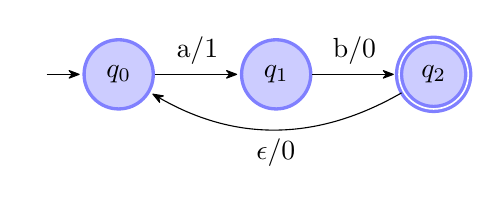
\begin{tikzpicture}[shorten >=1pt,node distance=2cm,on grid,>={Stealth[round]},
      every state/.style={draw=blue!50,very thick,fill=blue!20}, initial text=]

      \node[state,initial]            (q_0)                      {$q_0$};
      \node[state]                    (q_1) [right=of q_0]       {$q_1$};
      \node[state,accepting]          (q_2) [right=of q_1]       {$q_2$};

      \path[->] (q_0) edge              node      [above]           {a/1} (q_1)
      (q_1) edge              node      [above]           {b/0} (q_2)
      (q_2) edge [bend left]  node      [below]           {$\epsilon$/0} (q_0);
    \end{tikzpicture}
    \caption{$\aut_{(ab)\{1,100\}}$ with one register $r_1$ and $\theta = 1\leq r_1 \leq 100$}
    \label{fig:repetition}
  \end{figure}
\end{example}
The example \ref{eg:1} gives a general picture of constructing a CEFA for a regular expression: firstly, we build an NFA from the regex $\regex$
(e.g, To construct CEFA in example \ref{eg:1}, an NFA is construted with
transitions \{$q_0\xrightarrow{a} q_1\xrightarrow{b}q_2\xrightarrow{\epsilon}
  q_0\}$ initial state $q_0$, and accepting state $q_2$). Secondly, we extend NFA to CEFA by adding registers to $R$ and vector to each transition (e.g., the
register $r_1$ is added to store repetition times and add vector $\myvec{1}$ is set to transition $q_0\xrightarrow{a}q_1$ to update the repetition time). Finally, we set the
linear arithmetic $\theta$ carefully to restrict the accepted word to be
included in $\lan(\regex)$ (e.g., $\theta = 1\leq r_1\geq 100$ is set to
restrict the repetition times to $[1,100]$). Besides the repetition operation, other operations are non-trivial on CEFA. We individually discuss them in the following subsections.

\subsection{Non-nested Repetition}\label{subsec:rep}
Given a CEFA $\aut = (Q,\Sigma,\delta,I,F,\emptyset,true)$, the repetition operation $\{m,n\}$ on it is defined as a CEFA $\aut_{rep} = (Q, \Sigma, \delta', I, F, r_1, \theta')$ where: 
\begin{itemize}
  \item $r_1$ is the new register,
  \item $\delta'$ is composed by transitions $q\xrightarrow[\myvec{v}\cdot 0]{a} q'$ for all transitions $q\xrightarrow[\myvec{v}]{a} q' \in \delta$, and transitions $q_m\xrightarrow[0_{n}\cdot 1]{\epsilon} q_0$  for all $q_m\in F$ and $q_0\in I$,
  \item $\theta'$ is the linear arithmetic $m\leq r_1\leq n$ if all initial states are not accepting. Otherwise, $\theta'$ is the linear arithmetic $r_1\leq n$. 
\end{itemize} 
In the construction of $\aut_{rep}$, a new register $r_1$ is added to store the repetition times. The transition $q_m\xrightarrow[0_{n}\cdot 1]{\epsilon} q_0$ is added to update the repetition times. The linear arithmetic $\theta'$ is set to restrict the repetition times to $[m,n]$. Because arbitrary repetition times of empty string is still empty string, the value of $r_i$ need not be greater than $m$ when some initial states are accepting.\newline
Note that the given CEFA $\aut$ does not contain register. So the repetition operation on $\aut$ is non-nested.

\subsection{Concatenation}\label{subsec:con}
Given two CEFA $\aut_1 = (Q_1, \Sigma, \delta_1, I_1, F_1, R_1, \theta_1)$ and $\aut_2 = (Q_2, \Sigma, \delta_2,$ $I_2, F_2, R_2, \theta_2)$ with $R_1\cap R_2= \emptyset$ and $|R_1|=m,|R_2|=n$, the concatenation is defined as $\aut_{con}=(Q_1\cup Q_2, \Sigma, \delta', I_1, F_2, R_1\cdot R_2, \theta_1\wedge\theta_2)$ where $\delta'$ is composed by
\begin{itemize}
  \item $q_1\xrightarrow[\myvec{v_1}\cdot 0_n]{a} q_1'$ for each transition $q_1\xrightarrow[\myvec{v_1}]{a} q_1' \in \delta_1$,
  \item $q_2\xrightarrow[0_m\cdot\myvec{v_2}]{a} q_2'$ for each transition $q_2\xrightarrow[\myvec{v_2}]{a} q_2' \in \delta_2$,
  \item and $q_1\xrightarrow[0_{m+n}]{\epsilon} q_2$ for each $q_1\in F_1$ and $q_2 \in I_2$.
\end{itemize}
% \begin{figure}[h]
%   \centering
%   \begin{subfigure}{0.20\textwidth}
%     \begin{tikzpicture}[shorten >=1pt,node distance=2cm,on grid,>={Stealth[round]},
%       every fit/.style={draw,minimum height=2cm,minimum width=3.5cm,dashed},
%       every state/.style={draw=blue!50,minimum size = 0.1cm}, initial text=]
%       \node[state, initial]   (q_0) {};
%       \node[state, accepting]    (q_1) [right=of q_0] {};
%       \path[->] (q_0) edge [bend right] node [below] {$a/\myvec{v_1}$} (q_1);
%       \node [fit=(q_0) (q_1)] {$\cdots$};
%     \end{tikzpicture}
%     \caption{The CEFA $\aut_1$}
%   \end{subfigure}
%   \begin{subfigure}{0.20\textwidth}
%     \begin{tikzpicture}[shorten >=1pt,node distance=2cm,on grid,>={Stealth[round]},
%       every fit/.style={draw,minimum height=2cm,minimum width=3.5cm,dashed},
%       every state/.style={draw=blue!50,minimum size = 0.1cm}, initial text=]
%       \node[state, initial]   (q_0) {};
%       \node[state, accepting]    (q_1) [right=of q_0] {};
%       \path[->] (q_0) edge [bend right] node [below] {$a/\myvec{v_2}$} (q_1);
%       \node [fit=(q_0) (q_1)] {$\cdots$};
%     \end{tikzpicture}
%     \caption{The CEFA $\aut_2$}
%   \end{subfigure}
%   \begin{subfigure}{0.4\textwidth}
%     \begin{tikzpicture}[shorten >=1pt,node distance=2cm,on grid,>={Stealth[round]},
%       every fit/.style={draw,minimum height=2cm,minimum width=3.5cm,dashed},
%       every state/.style={draw=blue!50,minimum size = 0.1cm}, initial text=]
%       \node[state, initial]   (q_0) {};
%       \node[state]    (q_1) [right=of q_0] {};
%       \node[state]    (q_2) [right=of q_1] {};
%       \node[state, accepting]    (q_3) [right=of q_2] {};
%       \path[->]
%       (q_0) edge [bend right] node [below] {$a/\myvec{v_1}\cdot \red{0_n}$} (q_1)
%       (q_1) edge node [below] {$\red{0_{m+n}}$} (q_2)
%       (q_2) edge [bend right] node [below] {$a/\red{0_m}\cdot \myvec{v_2}$} (q_3);
%       \node [fit=(q_0) (q_1)] {$\cdots$};
%       \node [fit=(q_2) (q_3)] {$\cdots$};
%     \end{tikzpicture}
%     \caption{The concatenation of $\aut_1$ and $\aut_2$}
%   \end{subfigure}
%   \caption{Concatenation}
%   \label{fig:con}
% \end{figure}
The concatenation of two CEFAs is similar to the concatenation of two NFAs, except that the registers and its updates are also concatenated. 

% Figure \ref{fig:con} outlines the vector change on transitions when concatenating two CEFA. Without losing information, $\aut_{con}$ contains all registers in $\aut_1$ and $\aut_2$. Furthermore, $\aut_{con}$ update registers' value of $\aut_1$ and $\aut_2$ separately: $\aut_{con}$ only update registers of $R_1$ on the transitions of $\aut_1$ and update registers of $R_2$ on the transition of $\aut_2$. $\theta'$ is the conjunction of $\theta_1$ and $\theta_2$ to make sure all linear constraints in $\aut_1$ and $\aut_2$ are satisfiable.
\subsection{Intersection}\label{subsec:inter}
Given two CEFA $\aut_1 = (Q_1, \Sigma, \delta_1, I_1, F_1, R_1, \theta_1)$ and $\aut_2 = (Q_2, \Sigma, \delta_2,$ $I_2, F_2, R_2, \theta_2)$ with $R_1\cap R_2 = \emptyset$, the intersection is defined as $\aut_{inter} = (Q_1\times Q_2, \Sigma, \delta', I_1\times I_2, F_1\times F_2, R_1\cdot R_2, \theta_1\wedge \theta_2)$ where $\delta'$ is composed by
\begin{itemize}
  \item transitions $(q_1,q_2)\xrightarrow[\myvec{v_1}\cdot\myvec{v_2}]{a} (q_1',q_2')$ for  transition $q_1\xrightarrow[\myvec{v_1}]{a}q_1'$ and transition $q_2\xrightarrow[\myvec{v_2}]{a}q_2'$ exist individually in  $\delta_1$ and $\delta_2$.
\end{itemize}
% \begin{figure}[h]
%   \centering
%   \begin{subfigure}{0.20\textwidth}
%     \begin{tikzpicture}[shorten >=1pt,node distance=2cm,on grid,>={Stealth[round]},
%       every fit/.style={draw,minimum height=2cm,minimum width=3.5cm,dashed},
%       every state/.style={draw=blue!50,minimum size = 0.1cm}, initial text=]
%       \node[state, initial]   (q_0) {};
%       \node[state, accepting]    (q_1) [right=of q_0] {};
%       \path[->]
%       (q_0) edge [bend right] node [below] {$a$/$\myvec{v_1}$} (q_1)
%       (q_0) edge [bend left] node [above] {$b$/$\myvec{v_1}$} (q_1);
%       \node [fit=(q_0) (q_1)] {$\cdots$};
%     \end{tikzpicture}
%     \caption{The CEFA $\aut_1$}
%   \end{subfigure}
%   \begin{subfigure}{0.20\textwidth}
%     \begin{tikzpicture}[shorten >=1pt,node distance=2cm,on grid,>={Stealth[round]},
%       every fit/.style={draw,minimum height=2cm,minimum width=3.5cm,dashed},
%       every state/.style={draw=blue!50,minimum size = 0.1cm}, initial text=]
%       \node[state, initial]   (q_0) {};
%       \node[state, accepting]    (q_1) [right=of q_0] {};
%       \path[->]
%       (q_0) edge [bend right] node [below] {$a$/$\myvec{v_2}$} (q_1)
%       (q_0) edge [bend left] node [above] {$c$/$\myvec{v_2}$} (q_1);
%       \node [fit=(q_0) (q_1)] {$\cdots$};
%     \end{tikzpicture}
%     \caption{The CEFA $\aut_2$}
%   \end{subfigure}
%   \begin{subfigure}{0.4\textwidth}
%     \centering
%     \begin{tikzpicture}[shorten >=1pt,node distance=2cm,on grid,>={Stealth[round]},
%       every fit/.style={draw,minimum height=2cm,minimum width=3.5cm,dashed},
%       every state/.style={draw=blue!50,minimum size = 0.1cm}, initial text=]
%       \node[state, initial]   (q_0) {};
%       \node[state, accepting]    (q_3) [right=of q_0] {};
%       \path[->]
%       (q_0) edge [bend right] node [below] {$a$/\red{$\myvec{v_1}\cdot \myvec{v_2}$}} (q_3);
%       \node [fit=(q_0) (q_3)] {$\cdots$};
%     \end{tikzpicture}
%     \caption{The intersection of $\aut_1$ and $\aut_2$}
%   \end{subfigure}
%   \caption{Intersection}
%   \label{fig:inter}
% \end{figure}
The intersection of two CEFAs is similar to the intersection of NFA, except that the registers updates and linear arithmetic are also intersected.

\subsection{Union}\label{subsec:union}
Given two CEFA $\aut_1 = (Q_1, \Sigma, \delta_1, I_1, F_1, R_1, \theta_1)$ and $\aut_2 = (Q_2, \Sigma, \delta_2,$ $I_2, F_2, R_2, \theta_2)$ with $R_1\cap R_2 = \emptyset$ and $|R_1|=m,|R_2|=n$, the union is defined as $\aut_{union} = (Q_1\cup Q_2\cup\{q_0\}, \Sigma, \delta', \{q_0\}, F_1\cup F_2, R_1\cdot R_2\cdot (r_1, r_2), \theta')$ where $\delta'$ is composed by
\begin{itemize}
  \item transitions $q_0\xrightarrow[0_{m+n}\cdot(1,0)]{\epsilon}q_1$ for all $q_1\in I_1$,
  \item transitions $q_0\xrightarrow[0_{m+n}\cdot(0,1)]{\epsilon}q_2$ for all $q_2\in I_2$,
  \item transitions $q_1\xrightarrow[\myvec{v_1}0_{n+2}]{a} q_1'$ for all $q_1\xrightarrow[\myvec{v_1}]{a} q_1'\in \delta_1$,
  \item transitions $q_2\xrightarrow[0_m\myvec{v_2}0_2]{a} q_2'$ for all $q_2\xrightarrow[\myvec{v_2}]{a} q_2'\in \delta_2$.
\end{itemize}
$r_1$ and $r_2$ are new registers. $q_0$ is a new state where $q_0\not\in Q_1$ and $q_0\not\in Q_2$. Assume that $\theta  = (r_1>0\wedge\theta_1)\vee(r_2>0\wedge\theta_2)$, $\theta'$ is constructed differently in four cases:
\begin{itemize}
  \item both $I_1$ and $I_2$ do not contain accepting states: $\theta'$ = $\theta $;
  \item $I_1$ contains accepting states while $I_2$ does not: $\theta'$ = $\theta \vee (r_1==0\wedge r_2==0\wedge\theta_1)$;
  \item $I_2$ contains accepting states while $I_1$ does not: $\theta'$ = $\theta \vee (r_1==0\wedge r_2==0\wedge\theta_2)$;
  \item both $I_1$ and $I_2$ contain accepting states: $\theta'$ = $\theta \vee (r_1==0\wedge r_2==0\wedge(\theta_1\vee\theta_2))$;
\end{itemize}

% \begin{figure}[h]
%   \centering
%   \begin{subfigure}{0.20\textwidth}
%     \begin{tikzpicture}[shorten >=1pt,node distance=2cm,on grid,>={Stealth[round]},
%       every fit/.style={draw,minimum height=2cm,minimum width=3.5cm,dashed},
%       every state/.style={draw=blue!50,minimum size = 0.1cm}, initial text=]
%       \node[state, initial]   (q_0) {};
%       \node[state, accepting]    (q_1) [right=of q_0] {};
%       \path[->]
%       (q_0) edge [bend left] node [above] {$a$/$\myvec{v_1}$} (q_1);
%       \node [fit=(q_0) (q_1)] {$\cdots$};
%     \end{tikzpicture}
%     \caption{The CEFA $\aut_1$}
%   \end{subfigure}
%   \begin{subfigure}{0.20\textwidth}
%     \begin{tikzpicture}[shorten >=1pt,node distance=2cm,on grid,>={Stealth[round]},
%       every fit/.style={draw,minimum height=2cm,minimum width=3.5cm,dashed},
%       every state/.style={draw=blue!50,minimum size = 0.1cm}, initial text=]
%       \node[state, initial]   (q_0) {};
%       \node[state, accepting]    (q_1) [right=of q_0] {};
%       \path[->]
%       (q_0) edge [bend right] node [below] {$a$/$\myvec{v_2}$} (q_1);
%       \node [fit=(q_0) (q_1)] {$\cdots$};
%     \end{tikzpicture}
%     \caption{The CEFA $\aut_2$}
%   \end{subfigure}
%   \begin{subfigure}{0.4\textwidth}
%     \centering
%     \begin{tikzpicture}[shorten >=1pt,node distance=2cm,on grid,>={Stealth[round]},
%       every fit/.style={draw,minimum height=2cm,minimum width=3.5cm,dashed},
%       every state/.style={draw=blue!50,minimum size = 0.1cm}, initial text=]
%       \node[state, initial]   (q_0) {};
%       \node[state]   (q_1) [above right=of q_0] {};
%       \node[state, accepting]   (q_1') [right=of q_1] {};
%       \node[state]   (q_2) [below right=of q_0] {};
%       \node[state, accepting]   (q_2') [right=of q_2] {};
%       \path[->]
%       (q_0) edge node [left] {$\epsilon/\red{0_{m+n}\cdot(1,0)}$} (q_1)
%       (q_0) edge node [left] {$\epsilon/\red{0_{m+n}\cdot(0,1)}$} (q_2)
%       (q_1) edge [bend left] node [above] {$a$/\red{$\myvec{v_1}\cdot 0_{n+2}$}} (q_1')
%       (q_2) edge [bend right] node [below] {$a$/\red{$0_m\cdot \myvec{v_2}\cdot 0_2$}} (q_2');
%       \node [fit=(q_1) (q_1')] {$\cdots$};
%       \node [fit=(q_2) (q_2')] {$\cdots$};
%     \end{tikzpicture}
%     \caption{The union of $\aut_1$ and $\aut_2$}
%   \end{subfigure}
%   \caption{Union}
%   \label{fig:union}

% \end{figure}
To simulate the semantics of the union, we add transitions from $q_0$ to initial states of $\aut_1$ and $\aut_2$ to randomly choose one automaton. $r_1 > 0$ indicates we choose $\aut_1$ to run while $r_2 > 0$ indicates we choose $\aut_2$ to run. We should make sure the accepting condition is consistent. Therefore, the accepting condition $(r_1>0\wedge\theta_1)\vee(r_2>0\wedge\theta_2)$ is generated. Furthermore, the accepting run may stop at the new initial state $q_0$ with $\mathcal{V}(r_1) = 0, \mathcal{V}(r_2)=0$. It can only happen when some initial states of two given CEFAs are accepting. If some initial states of $\aut_1$ are accepting, the accepting condition $r_1=0\wedge r_2=0\wedge \theta_1$ is generated. Similarly, if some initial states of $\aut_2$ are accepting, the accepting condition $r_1=0\wedge r_2=0\wedge \theta_2$ is generated. Finally, the disjunction of all generated accepting conditions $\theta'$ is obtained to express the non-nondeterministic. 
\subsection{Complement}
Given a CEFA $\aut = (Q, \Sigma, I, F, \delta, \emptyset, true)$, the complement $\aut^c$ is defined as the CEFA $\aut^c = (Q, \Sigma, I, F^c, \delta, R, \theta^c)$ where $F^c = Q\setminus F$ and $\theta^c = \neg \theta$.
\subsection{Closure}
\subsection{Complement of Repetition and Nested Repetition}\label{subsec:comp}
As we mentioned,  CEFA 

\subsection{From Regex to CEFA} \label{subsec:regex2cefa}
\highlight{Basis}: The basis has three parts with empty registers and valid linear arithmetic, shown in Fig. \ref{fig:basis}. In part \ref{fig:basis:a}, we see how to handle the expression $\epsilon$. The language of the automaton is easily seen to be $\{\epsilon\}$ since the only path from the start state to an accepting state
is labeled $\epsilon$. Part \ref{fig:basis:b} gives the CEFA for a regular expression $\mathbf{a}$. The language of this CEFA consists of the single string $a$, which is also $\lan(\mathbf{a})$. Finally, part \ref{fig:basis:c} shows the construction for $\emptyset$. There are no paths from the initial state to the accepting state.
\begin{figure}[h]
  \centering
  \begin{subfigure}{0.3\textwidth}
    \centering
    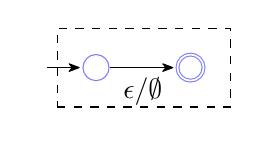
\begin{tikzpicture}[shorten >=1pt,node distance=1.2cm,on grid,>={Stealth[round]},
      every fit/.style={draw,minimum height=1.0cm,minimum width=2.2cm,dashed},
      every state/.style={draw=blue!50,minimum size = 0.1cm}, initial text=]
      \node[state, initial]   (q_0) {};
      \node[state, accepting]    (q_1) [right=of q_0] {};
      \path[->] (q_0) edge node [below] {$\epsilon/\emptyset$} (q_1);
      \node [fit=(q_0) (q_1)] {};
    \end{tikzpicture}
    \caption{}
    \label{fig:basis:a}
  \end{subfigure}
  \begin{subfigure}{0.3\textwidth}
    \centering
    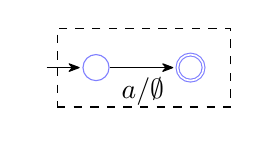
\begin{tikzpicture}[shorten >=1pt,node distance=1.2cm,on grid,>={Stealth[round]},
      every fit/.style={draw,minimum height=1.0cm,minimum width=2.2cm,dashed},
      every state/.style={draw=blue!50,minimum size = 0.1cm}, initial text=]
      \node[state, initial]   (q_0) {};
      \node[state, accepting]    (q_1) [right=of q_0] {};
      \path[->] (q_0) edge node [below] {$a/\emptyset$} (q_1);
      \node [fit=(q_0) (q_1)] {};
    \end{tikzpicture}
    \caption{}
    \label{fig:basis:b}
  \end{subfigure}
  \begin{subfigure}{0.3\textwidth}
    \centering
    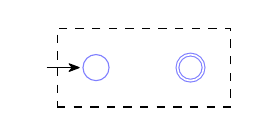
\begin{tikzpicture}[shorten >=1pt,node distance=1.2cm,on grid,>={Stealth[round]},
      every fit/.style={draw,minimum height=1.0cm,minimum width=2.2cm,dashed},
      every state/.style={draw=blue!50,minimum size = 0.1cm}, initial text=]
      \node[state, initial]   (q_0) {};
      \node[state, accepting]    (q_1) [right=of q_0] {};
      \node [fit=(q_0) (q_1)] {};
    \end{tikzpicture}
    \caption{}
    \label{fig:basis:c}
  \end{subfigure}
  \caption{The basis of the construction of a CEFA from extended regex}
  \label{fig:basis}
\end{figure}\\
\highlight{Induction}: Given the CEFA of the subexpression, we construct the CEFA in five cases:
\begin{enumerate}
  \item The expression is $\regex\{m,n\}$ for some smaller expression $\regex$. We can repeat the CEFA of $\regex$ with lower bound $m$ and upper bound $n$ as shown in section \ref{subsec:rep}.
  \item The expression is $\regex_1\cdot\regex_2$ for some smaller expression $\regex_1$ and $\regex_2$. We can concatenate the CEFA of $\regex_1$ and the CEFA of $\regex_2$ as shown in section \ref{subsec:con}.
  \item The expression is $\regex_1\times \regex_2$ for some smaller expression $\regex_1$ and $\regex_2$. We can intersect the CEFA of $\regex_1$ and the CEFA of $\regex_2$ as shown in section \ref{subsec:inter}.
  \item The expression is $\regex_1 + \regex_2$ for some smaller expression $\regex_1$ and $\regex_2$. We can union the CEFA of $\regex_1$ and the CEFA of $\regex_2$ as shown in section \ref{subsec:union}.
  \item The expression is $\regex*$ for some smaller expression $\regex$. We can construct the closure Star of the CEFA of $\regex$  as shown in section \ref{subsec:klee}.
  \item The expression is $\regex^C$ for some smaller expression $\regex$. We can construct the complement of the CEFA of $\regex$  as shown in section \ref{subsec:comp}
\end{enumerate}
\highlight{Special Case}: When the expression $\regex$ contains nested repetition, we firstly write $\regex$ to a new regex $\regex'$ without nested repetition. Then we build the CEFA of the new expression $\regex'$ by basis and induction steps.

\section{Solve String Constraints with Large Repetition Bound} \label{sec:solve}
Following the decision procedure defined in the paper \cite{atva2020}, we propose an efficient algorithm to solve string constraints with help of CEFA. Firstly, we replace all length operations $i=\strlen{x}$ to pre-images which are represented by CEFAs, and intersect these CEFAs to $lenAut_x$. Then for each term $x$, we generate CEFAs of all regular expressions $\regex$ in all terms $x\in \regex$, and intersect these CEFAs with $lenAut_x$ to get the final CEFA. Finally, we check whether each final CEFA is empty under the linear integer arithmetic $P$. If one of the final CEFAs is empty, the string constraints are unsatisfiable. Otherwise, the string constraints are satisfiable. The high-level algorithm is shown in the Algorithm \ref{alg:high}.\newline
The emptiness checking problem of CEFAs under linear integer arithmetic $P$ is theoretically pspace-complete\cite{atva2020}. To solve it efficiently for practical example, we add some heuristics. The details of the heuristics are shown in Algorithm \ref{alg:emptiness}.
% \pagebreak
\subsection{High-level algorithm}
\begin{algorithm}
  \caption{High-level algorithm}
  \label{alg:high}
  \begin{algorithmic}[1]
    \Require  Conjunction $\varphi$ of the form $x\in \regex$, and conjunction of linear integer arithmetic $P$ over string lengths
    \Ensure \emph{sat} or \emph{unsat}
    \Statex
    \ForAll{length operation $i = \strlen{x}$} \label{alg:high:line1}
      \State $lenAut_{x} \leftarrow \aut_{allstring}$ \label{alg:high:line2}
      \State Let $\aut_{i}$ be the pre-image of length operation with length $i$ \label{alg:high:line3}
      \State $lenAut_{x} \leftarrow lenAut_{x} \times \aut_{i}$ \label{alg:high:line4}
    \EndFor \label{alg:high:line5}
    \State $atomAuts \leftarrow \emptyset$ \label{alg:high:line6}
    \ForAll{string variables $x$ occurring in $\varphi$} 
    \State Let $S$ be the set of all regexes $\regex$ in all terms $x \in \regex$ 
    \State CEFA $\aut_x \leftarrow$ intersection of $lenAut_x$ and all CEFAs corresponding to regexes in $S$
    \If{$nfa(\aut_x)$ is empty} \label{alg:high:line5}
      \State \textbf{return} \emph{unsat}
    \EndIf
    \State $atomAuts \leftarrow atomAuts \cup \{\aut_x\}$ 
    \EndFor
    \If{$\algfun{isEmpty}(atomAuts, P)$ }
      \State \textbf{return} \emph{unsat}
    \Else 
      \State \textbf{return} \emph{sat}
    \EndIf
  \end{algorithmic}
\end{algorithm}
The pseudocode presented in Algorithm \ref{alg:high} outlines the framework of our solving process. The implemented details are eliminated for clarity. From line \ref{alg:high:line1} to line \ref{alg:high:line5}, we construct the CEFAs of all length operations occurring in the string constraints. The CEFA $lenAut_x$ is the automaton used to store length information on $x$. $lenAut_x$ is initiated to accept all strings at line \ref{alg:high:line2}. For each length operation $i = \strlen{x}$, we construct the pre-image of it at line \ref{alg:high:line3}, and intersect the pre-image to $lenAut_x$ at line \ref{alg:high:line4} to store length information. Note that the final $lenAut_x$ is the intersection of all pre-images so that it can store all length information on $x$.\newline
In the following steps, we call a CEFA to be \emph{atomic} if we will not operate it anymore. The set $atomAuts$ is the set of all atomic CEFAs for all terms $x$ occurring in the string constraints, and is initially empty at line \ref{alg:high:line6}. From line 7 to line 14, each atomic automaton in the set is constructed by intersecting the length automaton $lenAut_x$ to all CEFAs corresponding to the regex expressions with regard to string term $x$. If the NFA form of the atomic automaton is empty (i.e., the NFA accepts no word), we return $unsat$ directly because the NFA form is an over-approximation of CEFA. \newline
After obtaining the atomic CEFAs of all string terms, we check whether the atomic CEFAs are empty under the linear integer arithmetic $P$ at line 15. If the atomic CEFAs are empty under $P$, we return $unsat$. Otherwise, we return $sat$. The emptiness checking at line 15 is complex, and we discuss it detailly in the following subsection.\newline


\subsection{Emptyness Checking}
As mentioned, the emptiness checking problem of CEFA under linear integer arithmetic $P$ is theoretically pspace-complete \cite{atva2020}. In our previous research, we rewrote CEFA to an infinite system and used a model-checking tool \emph{NuSMV} to solve it. However, the previous method was not effictive enough. So we put forward a new method to solve it.\newline
As shown in Algorithm \ref{alg:emptiness}, We simplify the CEFAs at line 1 because the input CEFAs may have many transitions and registers. The purpose of the simplification is removing duplicated transitions and registers in the CEFA. After simplifying the input CEFAs, we try to find a solution by under-approximation at line 3. If we find a solution, we return $false$ at line 5 because the CEFAs under linear integer arithmetic $P$ are not empty. Otherwise, we try to find an unsat core by over-approximation at line 8.  If we discover an unsat core,  
we return $true$ at line 10 because we know that the CEFAs under $P$ are empty. Suppose that both under- and over-approximation do not make sense, we compute the Parikh images of the simplified CEFAs by algorithm in the paper \cite{parikh_2005}, and check if the Parikh images are satisfiable in conjunction with $P$ at line 12. The satisfiability implies non-emptiness directly. \newline
Note that the under-approximation program is executed many times until $MaxBound$ is reached. The details of simplification is shown in Algorithm \ref{alg:simplify}. The details of under- and over-approximation are shown in Algorithm \ref{alg:underApprox} and Algorithm \ref{alg:overApprox} respectively. The details of Parikh image computation are omitted for clarity.\newline
\begin{algorithm}
  \caption{ $\algfun{isEmpty}(auts, P)$}
  \label{alg:emptiness}
  \begin{algorithmic}[1]
    \Require CEFAs $auts$ and linear integer arithmetic $P$
    \Ensure $true$ or $false$
    \Statex
    \State $simpliAuts \leftarrow \algfun{simplify}(auts)$
    \For{$bound \gets 1, MaxBound$ }
      \State $\varphi_{under}\gets \algfun{underApprox}(simpliAuts, bound)$
      \If{$\varphi_{under}\wedge P$ is sat}
        \State \textbf{return} $false$
      \EndIf
    \EndFor
    \State $\varphi_{over}\gets \algfun{overApprox}(simpliAuts)$
    \If{$\varphi_{over}\wedge P$ is unsat}
      \State \textbf{return} $true$
    \EndIf
    \State $\varphi \gets \algfun{parikhImage}(simpliAuts)$
    \If{$\varphi\wedge P$ is unsat}
      \State \textbf{return} $true$
    \Else
      \State \textbf{return} $false$
    \EndIf
  \end{algorithmic}
\end{algorithm}

\subsection{Under-Approximation}
To solve the satisfiable instances of the emptiness checking problem, under-approximation procedure is come up. The main idea is exploring the CEFA deep-firstly. The string length bound the deep, and linear integer arithmetic is generated from low to high string length. This section only discusses the situation in where the string length bound is fixed. The details are shown in the Algorithm \ref{alg:underApprox}. Firstly, the linear integer arithmetic $\varphi_{under}$ is assigned to be false at line 1. Then for each CEFA, we enumerate all the accepted paths with lengths less than the bound and translate the paths to linear integer arithmetic. The linear integer arithmetic is in conjunction with $\varphi_{under}$ at line 4.
\begin{algorithm}
  \caption{$\algfun{underApprox}(auts, bound)$}
  \label{alg:underApprox}
  \begin{algorithmic}[1]
    \Require The CEFAs $auts$ and string length $bound$
    \Ensure The linear integer arithmetic $\varphi_{under}$ representing under-approximation of the register values of $auts$
    \Statex
    \State $\varphi_{under} \gets false$
    \For{$aut \in auts$}
      \State Suppose $aut = (Q, \Sigma, \delta, q_0, F, (r_1, \cdots, r_m), \theta)$
      \State $S_0 \gets \{(q_0, \myvec{0}_m)\}$
      \ForAll{path $q_0q_1\cdots q_{n}$ whose length is $bound$ and $\myvec{R}$ is the sum of the vectors on the path}
        \If{$q_{n}\in F$}
          \State $\varphi_{under} \gets \varphi_{under} \bigwedge_{i\in[1,m]} r_i = \myvec{R}(i)$
        \EndIf
      \EndFor
    \EndFor
    \State \textbf{return} $\varphi_{under}$
  \end{algorithmic}
\end{algorithm}
\subsection{Over-Approximation}
Sometimes when the bound reaches the maximum, the linear integer arithmetic $\varphi_{under}$ is still unsatisfiable. We must use over-approximation to solve the emptiness checking problem in this case. The main idea of over-approximation is to split each CEFA into sub-CEFAs, translate each sub-CEFA respectively, and finally in conjunction with the LIA of all sub-CEFAs. The details are shown in the Algorithm \ref{alg:overApprox}. Firstly, each CEFA is split into $n$ sub-CEFAs, where $n$ is the number of registers in the CEFA. The sub-CEFA has only one register. After simplifying each sub-CEFA by Algorithm \ref{alg:simplify}, the vector of each transition must be $\myvec{1}$. So the register value of each sub-CEFA equals the length of the accepted path. We apply the efficient construction of semilinear representations\cite{unary_nfa_2010} to get the linear integer arithmetic $\varphi_{over}$.
\begin{algorithm}
  \caption{$\algfun{overApprox}(auts)$}
  \label{alg:overApprox}
  \begin{algorithmic}[1]
    \Require CEFAs $auts$
    \Ensure Linear integer arithmetic $\varphi_{over}$
    \Statex
    \State $\varphi_{over} \gets true$
    \For{$aut \in auts$}
      \State Let $subAut$ be the sub-CEFA of $aut$ with only one register
      \State Let $subAut \gets \algfun{simplify}(subAut)$
      \State Let $\varphi_{subAut}$ be the linear integer arithmetic generated by efficient construction of semilinear representations
      \State $\varphi_{over} \gets \varphi_{over} \wedge \varphi_{subAut}$
    \EndFor
    \State \textbf{return} $\varphi_{over}$
  \end{algorithmic}
\end{algorithm}

\subsection{Simplification of CEFA}
The main purpose of simplification is to remove duplicated transitions and registers. In the emptiness checking Algorithm \ref{alg:emptiness}, the vectors on the transitions are meaningful while the letters on the transitions are not. So we see the alphabet of the CEFA as unary (i.e., the alphabet is $\{a\}$). Then the vector in the CEFA is seen as the letter in the NFA, and the vector $\myvec{0}_n$ is seen as $\epsilon$. Based on the homomorphism between NFA and CEFA, we determinate and minimize \cite{aut_hopcraft} the CEFA by vector firstly. Then we merge the registers having the same updating at all transitions. The main simplification framework is shown in Algorithm \ref{alg:simplify}. 
\begin{algorithm}
  \caption{$\algfun{simplify}(auts)$}
  \label{alg:simplify}
  \begin{algorithmic}[1]
    \Require CEFAs $auts$
    \Ensure Simplified CEFAs $simpliAuts$
    \Statex
    \State $simpliAuts \gets \emptyset$
    \For{$aut \in auts$}
      \State $aut \gets \algfun{determinizeByVec}(aut)$
      \State $aut \gets \algfun{minimizeByVec}(aut)$
      \State $aut \gets \algfun{mergeRegisters}(aut)$
      \State $simpliAuts \gets simpliAuts \cup \{aut\}$
    \EndFor
    \State \textbf{return} $simpliAuts$
  \end{algorithmic}
\end{algorithm}


\section{Implementation and Experiment} \label{sec:imp}
% % TODO: Implementation and experiment result
TODO
\subsection{Overall Evaluation of Experiment}
tools: cvc5, z3str3, z3str3re, z3-trau, ostrich
benchmark: total benchmark

\subsection{Experimental Details}
tools: cvc5, z3str3, z3str3re, z3-trau, ostrich
benchmmark:
\begin{itemize}
  \item Small Count: the sum of upper bounds on the repetition operator is less than 50
  \begin{itemize}
    \item z3str3re-bench
    \item regexlib
    \item stackoverflow
    \item ReDos-bench
  \end{itemize}
  \item Large Count: the sum of upper bounds on the repetition operator is greater than 50
  \begin{itemize}
    \item z3str3re-bench
    \item regexlib
    \item stackoverflow
    \item ReDos-bench
  \end{itemize}
\end{itemize}


\subsection{Analysis of All Algorithms}
tools:
\begin{itemize}
  \item ostrich-baseline: the origin ostrich syntactically unwind all repetition operators.
  \item ostrich-new: the most efficient ostrich which using CEFA and all heuristics
  \item ostrich-without-under: without under-approxiamtion
  \item ostrich-without-over: without over-approximation
  \item ostrich-without-simplification: without simplification of CEFA
  \item ostrich-without-rapidly-finding-string: without context-aware finding string
\end{itemize}


\section{Conclusion and Future Work} \label{sec:conclu}
In this paper, we aim to solve the string constraints with large repetition time efficiently. A new automaton model CEFA is proposed to reduce the search space. Many basic operations on CEFA are non-trivial and we should formal them carefully. Moreover, we extend the algorithm in the paper \cite{atva2020} with heuristics such as under- and over-approximation. The implementation of the algorithm is done on string solver ostrich. The extensive empirical comparison against z3 over a large and diverse benchmark shows the power of our model and algorithm. In the future, we plan to explore the way to solve nested repetition and use CEFA to solve more string operations.

%%
%% The next two lines define the bibliography style to be used, and
%% the bibliography file.
\bibliographystyle{ACM-Reference-Format}
\bibliography{ref}

\end{document}

%%
%% End of file `sample-sigconf.tex'.
